

\section{Method}


\newpage

\subsection{Optimal Finger Dimensions}
Material properties:
\begin{table}[h!]
\centering
		\caption{Material properties according to Ultimaker technical data sheets.}
		\label{tab:mat_props}
	\begin{tabular}{lrrl}
		& PLA & PP & unit \\
		$E$ & {1820} &  {220} & \si{\mega\pascal} \\
		$\sigma_\text{yield}$ & {37}& {8.7} & \si{\mega\pascal} \\
		%$\sigma_\text{break}$ & {37}& ? & \si{\percent} \\
		$\epsilon_\text{yield}$ & {3.1}& {18} & \si{\percent} \\
		%$\epsilon_\text{break}$ & {3.1} &  $ > 300$  & \si{\percent} \\
		%$\sigma_\text{bend}$ & {78} & {13} & \si{\mega\pascal} \\
		%$E_\text{bend}$ & {2490}  & {305} & \si{\mega\pascal} \\
	\end{tabular}
\end{table}


When any structure would fail by breakage or plastic deformation,
the structure could be enhanced by reinforcing the location where that fault would happen.
Our interlocking structure consists of beams of two materials.
Reinforcing the beams of one material means that we reduce beams of the other material.
If we consider beams of a homogeneous width then the respective widths of the beams is subject to optimization.
The width ratio is optimal when both materials would fail under the same load.
The optimized ratio between PLA and PP is therefore
$
A^\text{PP} / A^\text{PLA} = \sigma^\text{PLA}_\text{yield} / \sigma^\text{PP}_\text{yield}  \approx 4.3
$.
See \cref{tab:mat_props}.
If we choose the width of the PLA beams to be two standard lines wide, \SI{0.7}{\milli\meter}, then the PP beams should be \SI{3.0}{\milli\meter}.




The height of the beams is irrelevant to the optimization.
Only when the beams are a lot higher than the layer thickness does a new failure mode come into play where the beams in the orthogonal directions shear off each other.
Given that the ultimate shear stress is approximately half the ultimate tensile stress,
this failure mode plays a role when the contact area between the beams is half the cross sectional area of a beam.
However, the width of the beams is in the order of twice the nozzle size, whereas the layer height is in the order of a quarter of the nozzle size.
If we keep the beams as high as two layers the shearing failure mode will not take effect.
\begin{align*}
	\sigma_\text{tensile} &= \frac{F}{h w_\text{finger}} \\
	\sigma_\text{shear} &= \frac{F}{w_\text{beam} w_\text{finger}} \\
	\sigma_\text{ultimate shear}^m &\in \left(50\%,100\%\right) \sigma_\text{ultimate tensile}^m \text{ for any material $m$} \\
	h &< \nicefrac12 w_\text{beam} \\ 
\end{align*}

\subsection{Optimal Varying Finger Width}

Let's consider a PLA finger which crosses $N$ beams, which is allowed to vary in width.
See \cref{force_distribution}.
In case one segment would have a higher stress than the others then that one would be the weakest link, so in the optimal structure all segments have the same stress $\sigma$.
However, when the two materials are different it is not possible to optimize the structure such that both links will break at the same time.
Since the links of the fingers are (inter)locked at either end the elongation of the link will be shared among both materials, so the material with the lowest value for elongation at break will always be the link that breaks first.
We therefore set the stress along all links with the material with the lower elongation at break at the yield stress, while setting only the stress of the base link of the other material at its respective yield stress;
the stresses of the other links will be lower, because they are constrained.

Given an extension $\epsilon$ of a link consisting of two parallel beams $a$ and $b$ which are connected at the ends:
\begin{align*}
	E &\equiv \frac{\sigma}{\epsilon} \\
	\sigma &= E \epsilon \\
	\frac{\sigma^a}{\sigma^b} &=  \frac{E^a \epsilon}{E^b \epsilon} 
	= \frac{E^a}{E^b}  \\
	\\
	\sigma &\equiv \frac{F}{A} \\
	F &= \sigma A = E \epsilon hw \\
	\frac{F^a}{F^b} &= \frac{E^a \epsilon h w^a}{E^b \epsilon h w^b}
	= \frac{E^a w^a}{E^b w^b} \\
	F^b &= F^a \frac{E^b}{E^a} \frac{w^b}{w^a} \\
\end{align*}
So the actual distribution of stresses between the two beams depends on their relative Young's moduli and the total elongation.
However, the total elongation depends on the widths of the beams.

Let's assume that material $a$ yields (or breaks) at a lower strain value
and that $a$ yields before $b$ yields (?), i.e. $\sigma^a_{\text{ yield}} < \sigma^b_{\text{ yield}} \nicefrac{E^a}{E^b}$.
Then the total strain when the link fails is determined by $a$.


In general:
\iffalse
\begin{align*}
    \sigma_x^m &= \frac{F_x^m}{w_x^m h}\\
	w &= w_x^a + w_{N+1-x}^b \\
	F_1^a &= F_1^b = F_x^a + F_{N+2-x}^b \\
	F_1^a &= F_1^b = F_{N+2-x}^b \frac{E^a}{E^b} \frac{w_x^a}{w_{N+2-x}^b} + F_{N+2-x}^b \\
	F_1^b &= F_{N+2-x}^b \left( 1 + \frac{E^a}{E^b} \frac{w_x^a}{w_{N+2-x}^b} \right) \\
	w_1^b \sigma_1^b &= w_{N+2-x}^b \sigma_{N+2-x}^b \left( 1 + \frac{E^a}{E^b} \frac{w_x^a}{w_{N+2-x}^b} \right) \\
	w_1^b &= \frac{\sigma_{N+2-x}^b}{\sigma_1^b} \left( w_{N+2-x}^b + \frac{E^a}{E^b} w_x^a \right) \\
\end{align*}
This isn't going anywhere, because there's no specific relationship for $\frac{\sigma_{N+2-x}^b}{\sigma_1^b}$.
\fi

\begin{align*}
    \sigma_x^m &= \frac{F_x^m}{w_x^m h}\\
    w &= w_x^a + w_{N+1-x}^b \\
    F_1^a &= F_1^b = F_x^a + F_{N+2-x}^b \\
    F_1^a &= F_1^b % = F_x^a + F^a_x \frac{E^b}{E^a} \frac{w^b_{N+2-x}}{w^a_x} \\
     = F_x^a \left( 1 + \frac{E^b}{E^a} \frac{w^b_{N+2-x}}{w^a_x} \right) \\
    % w_1^a h \sigma_1^a &= w_1^b h \sigma_1^b = w_x^a h \sigma_x^a + w_{N+2-x}^b h \sigma_{N+2-x}^b \\
    w_1^a \sigma_1^a &= w_1^b \sigma_1^b = w_x^a \sigma_x^a \left( 1 + \frac{E^b}{E^a} \frac{w^b_{N+2-x}}{w^a_x} \right) \\
    %&= w_x^a \sigma_x^a + w_x^a \sigma_x^a \frac{E^b}{E^a} \frac{w^b_{N+2-x}}{w^a_x} \\
    &= w_x^a \sigma_x^a + \sigma_x^a \frac{E^b}{E^a} w^b_{N+2-x} \\
    w_1^a &= w_x^a \frac{\sigma_x^a}{\sigma_1^a} + \frac{\sigma_x^a}{\sigma_1^a} \frac{E^b}{E^a} w^b_{N+2-x} \\
    %w_1^a \sigma_1^a &= w_1^b \sigma_1^b = w_x^a \sigma_x^a + w_{N+2-x}^b \sigma_{N+2-x}^b \\
    w_N^b &= w - w_1^a =  w_x^a + w_{N+1-x}^b  -  w_x^a \frac{\sigma_x^a}{\sigma_1^a} - \frac{\sigma_x^a}{\sigma_1^a} \frac{E^b}{E^a} w^b_{N+2-x} \\
    &= w_x^a \left( 1 - \frac{\sigma_x^a}{\sigma_1^a} \right) + w_{N+1-x}^b - \frac{\sigma_x^a}{\sigma_1^a} \frac{E^b}{E^a} w^b_{N+2-x} \\
\end{align*}

If material $a$ will fail first then the optimal structure has the same stress for material $a$ in each beam, i.e. $\sigma_x^a = \sigma_1^a$.

\begin{align*}
	w_N^b &= w_{N+1-x}^b - \frac{E^b}{E^a} w^b_{N+2-x} \\
	w_N^b &= w_{x}^b - \frac{E^b}{E^a} w^b_{x+1} \\
	w_{x}^b &= w_N^b + \frac{E^b}{E^a} w^b_{x+1} \\
	%\\
	%% x = N - 1
	%w_{N-1}^b &= w_N^b + \frac{E^b}{E^a} w^b_{N} \\
	%&= w_N^b \left( 1 + \frac{E^b}{E^a} \right) \\
	%\\
	%% x = N - 2
	%w_{N-2}^b &= w_N^b + \frac{E^b}{E^a} w^b_{N-1} \\
	%&= w_N^b + \frac{E^b}{E^a} w_N^b \left( 1 + \frac{E^b}{E^a} \right) \\
	%&= w_N^b \left( 1 + \frac{E^b}{E^a} \left( 1 + \frac{E^b}{E^a} \right) \right) \\
	%&= w_N^b \left( 1 + \frac{E^b}{E^a} + \left(\frac{E^b}{E^a} \right)^2 \right) \right) \\
	%\\
	%% x = N - 3
	%w_{N-3}^b &= w_N^b + \frac{E^b}{E^a} w^b_{N-2} \\
	%&= w_N^b + \frac{E^b}{E^a} w_N^b \left( 1 + \frac{E^b}{E^a} \left( 1 + \frac{E^b}{E^a} \right) \right) \\
	%&= w_N^b \left( 1 + \frac{E^b}{E^a} \left( 1 + \frac{E^b}{E^a} \left( 1 + \frac{E^b}{E^a} \right) \right) \right) \\
	%&= w_N^b \left( 1 + \frac{E^b}{E^a} + \left(\frac{E^b}{E^a} \right)^2  + \left(\frac{E^b}{E^a} \right)^3 \right) \right) \\
	%\\
	\dots \\
	%w^b_{N-x} &= w^b_N \left( \left(\frac{E^b}{E^a}\right)^0 + \dots + \left(\frac{E^b}{E^a}\right)^x \right) \\
	w^b_{N-x} &= w^b_N \sum\limits_{i=0}^x \left(\frac{E^b}{E^a}\right)^i \\
\end{align*}

We will optimize the structure such that material $b$ will break at the base at the same point as material $a$ break anywhere along the chain, i.e. $\sigma^b_1 = \sigma^b_\text{yield}$ and $\sigma^a  = \sigma^a_\text{yield}$.

\begin{align*}
	%\sigma_x^m &= \frac{F_x^m}{w_x^m h}\\
	h w_1^a &= \frac{F_1^a}{\sigma^a} \\
	%&= \frac{F_1^b}{\sigma_1^b} \frac{\sigma^b_\text{yield}}{\sigma^a_\text{yield}}\\
	&= w_1^b h \frac{\sigma^b_\text{yield}}{\sigma^a_\text{yield}}\\
	w_1^a &= w_1^b \frac{\sigma^b_\text{yield}}{\sigma^a_\text{yield}}\\
\end{align*}


Let's consider the case for $N=2$, $a$ is PLA and $b$ is PP.

\begin{align*}
	w_1^\text{PLA} &= w_1^\text{PP} \frac{\sigma^\text{PP}_\text{yield}}{\sigma^\text{PLA}_\text{yield}} = w_1^\text{PP} \frac{8.7}{37} \\
	w^\text{PP}_1 &=  w_2^\text{PP} \left( 1 + \frac{E^\text{PP}}{E^\text{PLA}}  \right) \\
	&=  w_2^\text{PP} \left( 1 + \frac{220}{1820}  \right) \\
	\\
	w_1^\text{PLA} &= 1.1 \text{ (just below $3\times$ nozzle size)}\\
	w_1^\text{PP} &= 4.68 \\
	w_2^\text{PP} &= 4.17 \\
	w &= 5.27 \\
	w_2^\text{PLA} &= 0.60 \\
\end{align*}

To verify:
\begin{align*}
	\frac{w_2^\text{PLA}}{w_1^\text{PP}} &= \frac{F^\text{PLA} E^\text{PP}}{F^\text{PP} E^\text{PLA}} \\
	\\
	\frac{F_\text{PLA}}{F_\text{PP}} &= \frac{E_\text{PLA} w_\text{PLA}}{E_\text{PP} w_\text{PP}} \\
\end{align*}

\iffalse

\begin{figure}
	\centering
	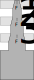
\includegraphics[height=.5\columnwidth]{sources/method/stress_distribution.pdf}
	\caption{Force distribution along a beam with varying width.}
	\label{force_distribution}
\end{figure}

\fi

